\documentclass[11pt,a4paper]{article}
\usepackage{tikz}
\usetikzlibrary{arrows.meta,positioning}
\usepackage{tabularx}
\usepackage{amsmath,amssymb,amsthm}
\usepackage{geometry}
\geometry{margin=1in}
\usepackage{hyperref}
\usepackage{graphicx}
\usepackage{setspace}
\onehalfspacing

\title{\textbf{Paper B-07: Logistics and Supply-Chain Dynamics:\\ A Constraint-Driven Flux Dynamics (CDFD) Perspective}}
\author{Steve Bico Mujjabi, MD\\
\small Independent Researcher\\
\small Founder, Vura Labs\\
\small Kampala, Uganda\\
\small ORCID: 0009-0001-0556-5516}
\date{August 2026}

\begin{document}
\maketitle

% BEGIN SHARED-METHODS POINTER
\noindent\textit{Shared Part IV notation and evidence boundaries are defined in \path{PART_IV_METHODS_AND_CLAIM_BOUNDARY.md}. This paper states only its local observables, comparison, and failure conditions.}
% END SHARED-METHODS POINTER


\begin{abstract}
This paper develops a falsifiable CDFD/AFL model of Logistics. It maps orders, shipments, materials, and customer demand to driving flux $\Phi$, vehicle, warehouse, port, labor, and information capacity to active constraint $C$, rerouting, inventory, substitution, prioritization, and coordination to responsiveness $S$, and contracts, inventories, path dependence, and disruption history to structural memory $M_s$. The target outcome is lead time, fill rate, cost, shortage, and recovery, tested against shipment traces, inventory records, network maps, lead times, and disruption logs. The paper treats universality as a shared model architecture rather than an assertion that unlike systems have the same material mechanism. It states the negative result that would make the mapping unnecessary and places the domain claim inside the cumulative CDFD programme and its reproducible runtime boundary.
\end{abstract}
% BEGIN CONSOLIDATION SCOPE
\section*{Consolidation Scope and Provenance}
This consolidated paper incorporates the logistics and supply-chain scopes formerly carried by Papers B-07 and D-11. Inventory, transport, supplier disruption, and bullwhip effects are candidate measurable mechanisms, not consequences of shared notation.
% END CONSOLIDATION SCOPE


\section{Introduction}

A supply chain is a physical transport network. Ore is mined in one hemisphere, processed in another, and consumed globally. To maximize profit, corporations have spent decades eliminating warehouses and stockpiles, relying on "just-in-time" (JIT) delivery.

In thermodynamic terms, JIT eliminates all buffer capacity from the system. It creates a network that is incredibly fast and efficient under perfect conditions but possesses zero topological elasticity. Under CDFD, this is a system balanced on a razor's edge, predicted here to be vulnerable to catastrophic failure upon the introduction of turbulence.

\section{The Logistical Adaptive Surface}
We evaluate supply chain networks using the Adaptive Operating Ratio:
\begin{equation}
    \Psi_s = \left( \frac{\Phi}{C} \right) \cdot S \cdot M_s
\end{equation}

For a specific logistical node (e.g., a major shipping port):
\begin{itemize}
    \item \textbf{Flux ($\Phi$)}: The volume of cargo containers or tonnage of goods arriving and departing daily.
    \item \textbf{Constraint ($C$)}: The physical unloading capacity of the cranes, labor availability, customs friction, and canal width restrictions.
    \item \textbf{Responsiveness ($S$)}: The available warehouse buffer space and the ability to dynamically reroute ships to alternative ports.
    \item \textbf{Memory ($M_s$)}: Fixed, long-term shipping contracts and consolidated mega-vessel dependencies. High memory locks the global shipping topology into a few rigid, highly efficient corridors, eliminating alternative pathways.
\end{itemize}

\subsection{The Ischemia of Just-In-Time Logistics}
A JIT supply chain intentionally drives responsiveness $S$ (buffer stock) to zero to save money. To maintain $\Psi_s \approx 1$, the flow $\Phi$ and the constraint $C$ must remain absolutely constant.

If a single major constraint spikes---such as a ship grounding in a critical canal or a sudden labor strike at a mega-port---$C \to \infty$ for that specific node. Because $S \approx 0$ and $M_s$ is locked (ships cannot easily reroute or unload elsewhere), the adaptive ratio for the entire global segment plummets to $\Psi_s \ll 1$.

The flux $\Phi$ backs up. Ships idle in the ocean. Factories on the other side of the planet halt production because they lack buffer inventory. The localized blockage induces a global topological stroke. The system's failure to maintain structural elasticity results in a complete cessation of macroscopic thermodynamic throughput.



\section{Measurement Layer}

% BEGIN PART IV MAJOR CROSS-DOMAIN UPGRADE
\section{Cross-Domain Model Upgrade: Mechanism, Scale, and Tests}

\subsection{Observable Translation}

The paper-specific translation begins with an observable chain rather than a
verbal analogy. For Logistics, the proposed drive is orders, shipments, materials, and customer demand.
The active limitation is vehicle, warehouse, port, labor, and information capacity. Responsiveness is carried by
rerouting, inventory, substitution, prioritization, and coordination, while retained state is represented by
contracts, inventories, path dependence, and disruption history. The outcome to explain is lead time, fill rate, cost, shortage, and recovery.

\begin{table}[htbp]
\centering
\small
\caption{Operational CDFD/AFL map for Paper B-07.}
\begin{tabularx}{\textwidth}{|l|X|X|}
\hline
\textbf{Term} & \textbf{Paper-specific observable meaning} & \textbf{Measurement question} \\
\hline
$\Phi$ & orders, shipments, materials, and customer demand & What rate, load, gradient, or demand enters the focal system? \\
\hline
$C$ & vehicle, warehouse, port, labor, and information capacity & Which measured bottleneck limits transfer, function, or recovery? \\
\hline
$S$ & rerouting, inventory, substitution, prioritization, and coordination & Which process changes effective capacity or reroutes the load? \\
\hline
$M_s$ & contracts, inventories, path dependence, and disruption history & Which retained state makes equal present loads produce different futures? \\
\hline
$Y$ & lead time, fill rate, cost, shortage, and recovery & Which outcome is predicted out of sample, with uncertainty? \\
\hline
\end{tabularx}
\end{table}

\begin{figure}[htbp]
\centering
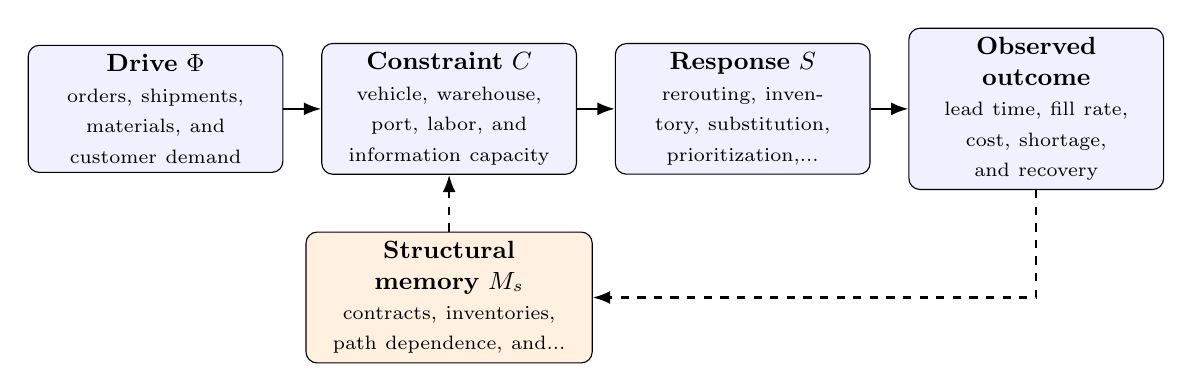
\begin{tikzpicture}[
    node distance=0.48cm,
    every node/.style={font=\small},
    box/.style={draw, rounded corners, align=center, minimum height=1.45cm, text width=3.0cm, fill=blue!6},
    memory/.style={draw, rounded corners, align=center, minimum height=1.25cm, text width=3.4cm, fill=orange!12},
    flow/.style={-{Latex[length=2.2mm]}, thick},
    feedback/.style={-{Latex[length=2.2mm]}, thick, dashed}
]
\node[box] (drive) {\textbf{Drive $\Phi$}\\\scriptsize orders, shipments, materials, and customer demand};
\node[box, right=of drive] (constraint) {\textbf{Constraint $C$}\\\scriptsize vehicle, warehouse, port, labor, and information capacity};
\node[box, right=of constraint] (response) {\textbf{Response $S$}\\\scriptsize rerouting, inventory, substitution, prioritization,...};
\node[box, right=of response] (outcome) {\textbf{Observed outcome}\\\scriptsize lead time, fill rate, cost, shortage, and recovery};
\node[memory, below=0.72cm of constraint] (memory) {\textbf{Structural memory $M_s$}\\\scriptsize contracts, inventories, path dependence, and...};
\draw[flow] (drive) -- (constraint);
\draw[flow] (constraint) -- (response);
\draw[flow] (response) -- (outcome);
\draw[feedback] (outcome.south) |- (memory.east);
\draw[feedback] (memory.north) -- (constraint.south);
\end{tikzpicture}
\caption{Paper B-07 observable CDFD/AFL architecture for Logistics. Solid arrows give the proposed forward chain; dashed arrows make history-dependent feedback explicit.}
\label{fig:b07-architecture}
\end{figure}

\subsection{Paper-Specific Causal Hypothesis}

For this paper, the hypothesized causal sequence is specific. A change in
orders, shipments, materials, and customer demand arrives faster than rerouting, inventory, substitution, prioritization, and coordination can compensate.
This raises or redistributes vehicle, warehouse, port, labor, and information capacity. If the load persists,
the retained state encoded by contracts, inventories, path dependence, and disruption history changes the next response, so a later event of equal
magnitude can produce a different trajectory in lead time, fill rate, cost, shortage, and recovery. The
scientific task is to estimate that sequence against the best ordinary model of
the domain, not merely to redescribe the outcome after it occurs.

\subsection{Cross-Scale Translation Without Mechanistic Erasure}

For the engineered systems family, the cross-domain translation compares demand, designed capacity, feedback control, dependency topology, and accumulated technical state. The strongest engineering use is prospective: the mapping must identify a bottleneck, a control action, or a recovery signature before the failure occurs. \cite{BarabasiAlbert1999,WattsStrogatz1998,Shannon1948,BakTangWiesenfeld1987}
The required scale declaration for this paper is hours to decades; parcels to global trade networks. At short
scales, the key question is whether the incoming drive is transmitted,
buffered, or diverted. At intermediate scales, response changes effective
capacity and network exposure. At long scales, retained structure can alter the
state space itself. A result is genuinely cross-scale only when the aggregation
rule is stated and the same conclusion is not an artifact of averaging.

\subsection{Evidence Ladder and Discriminating Tests}

\begin{table}[htbp]
\centering
\small
\caption{Evidence ladder for Paper B-07. Each rung can fail independently.}
\begin{tabularx}{\textwidth}{|p{0.17\textwidth}|X|X|}
\hline
\textbf{Test} & \textbf{Design} & \textbf{Discriminating result} \\
\hline
Proxy audit & Measure shipment traces, inventory records, network maps, lead times, and disruption logs and preregister how each record maps to $\Phi$, $C$, $S$, $M_s$, and $Y$. & The mapping fails if proxies are non-identifiable, circular, or change meaning across cases. \\
\hline
Load ramp & Apply or observe a supplier or corridor loss during a demand surge while estimating the dominant constraint and response time. & A threshold claim requires a reproducible nonlinear change and uncertainty bounds, not a visually chosen breakpoint. \\
\hline
Recovery and memory & Match present load across units with different histories, then compare recovery paths. & The memory claim requires history-dependent divergence after current conditions are controlled. \\
\hline
Model comparison & Compare the baseline domain model with and without the CDFD/AFL state variables using held-out data. & The paper's stated falsifier is: memory and topology terms do not improve shortage or recovery prediction. \\
\hline
\end{tabularx}
\end{table}

\subsection{Research Programme and Boundary Conditions}

The immediate research programme has four steps. First, construct a documented
dataset from shipment traces, inventory records, network maps, lead times, and disruption logs and retain raw units before normalization.
Second, fit a baseline domain model and report its calibration and out-of-sample
error. Third, add the smallest identifiable CDFD/AFL state extension and test
whether it improves prediction of lead time, fill rate, cost, shortage, and recovery. Fourth, repeat the
analysis across the declared scale range and publish negative cases as part of
the cross-domain translation audit.

% END PART IV MAJOR CROSS-DOMAIN UPGRADE

\section{Conclusion}
Supply chains are subject to a comparable flow problem to biological circulatory systems. A biological organism maintains fat reserves and redundant arteries (high $S$, low $M_s$) precisely to survive localized trauma. By analyzing global logistics through CDFD, we model the hypothesis that economic efficiency must be balanced with topological elasticity; otherwise, the network predicts its own eventual collapse.
\section*{Conflict of Interest} The author declares no conflict of interest.
\section*{Data Availability}
Part-specific runtime diagnostics are under each Part's \path{outputs/} directory.

Release-wide code: \path{Part_E_Synthesis/supplementary/}.

Generated summaries: \path{Part_E_Synthesis/outputs/}.

Figures: \path{Part_E_Synthesis/figures/}.


\section{Reference Layer}
\bibliographystyle{plain}
\bibliography{universal_afl_references}
\end{document}
